\chapter{\emph{\arr Project}: Torchelie}
\label{chap:tch}

\section{Introduction}

Back in Montréal, working for JSALT2019 in order to publish \cite{jsaltvq}, I wanted to gather all the deep learning related code I wrote so far for my thesis. The initial motivation to realize this project was clear: while deep learning code is often short to write, it is also extremely easy to get wrong, and even harder to diagnose and debug. In standard software engineering, most mistakes end up crashing the application or raising exceptions, making them obvious to uncover. In deep learning, they damage the results, often in very subtle ways.

Besides, many code bases would share common patterns: training and testing loops, alternating training for G and D in \acp{GAN}, measuring accuracy, layers or blocks, etc. In most public code, the training code is often made of raw for-loop instrumented with many ifs, and as the need to monitor new quantities grow, the code gets harder to maintain and error prone. As we try new incremental ideas, the ifs switches grow out of hand, readability suffers, and more bugs arise.

Torchélie is a software engineering take to tackle this problem and provide tools to build both experiments and production-ready code that is fast to write and easy to maintain, from battle tested building blocks. It is based on PyTorch that it extends.

Torchélie is a twofold contribution:
\begin{enumerate}
    \item first, as a library and toolbox for pytorch, providing many utilities. We aim to mimic PyTorch's style as close as possible, hoping to make it a seamless experience;
    \item second, as a set of design principles that can be followed even outside of Torchélie in order to ease iterative development.
\end{enumerate}

\section{Overview}

The first contribution Torchélie brings is a Python package based on PyTorch that contains multiple tools extending Pytorch horizontally:

\paragraph{\texttt{torchelie.datasets}} implements new datasets, new dataset transforms, and dataset utils. It contains utilities like \texttt{FastImageFolder} which caches pytorch's \texttt{ImageFolder} file list, making big datasets loading much faster; \texttt{PairedDatasets} sampling pairs from two datasets at a time, which is useful for tasks like image translation or augments like Mixup; \texttt{MixupDataset} which samples from a dataset and uses Mixup to augment the sampled image and its classification target; \texttt{Subset} which allows using only a random (but reproducible) subset of dataset, quantified either as a fraction or a number of samples. It also provides datasets loaders and downloaders such as \texttt{MS1M} which is able to load MS1M despite its file format encoded for MXnet, \texttt{Pix2PixDataset} loading from NVidia's servers the datasets used for Pix2Pix \cite{pix2pix}, \texttt{Imagenette}, and \texttt{Imagewoof}.

\paragraph{\texttt{torchelie.distributions}} adds Logistic distribution, LogisticMixture, GaussianMixture and Truncated Normal to \texttt{torch.distributions}, used mainly in PixelCNN(++) \cite{pixelcnn,pixelcnn++}.

\paragraph{\texttt{torchelie.loss}} contains many losses and regularizers, noticeably for \acp{GAN} (Hinge loss for BigGAN \cite{biggan}, R1 regularizer from \cite{R1}, R0 regularizer from \cite{r0}, WGAN loss from \cite{wgangp}), face recognition (\texttt{AdaCos} \cite{adacos}, \texttt{ArcFace} \cite{arcface}) and style transfer. It implements the \texttt{BitemperedLoss} from \citet{Bitempered} that is said to be more robust to label noise, \texttt{DeepDreamLoss} from \citet{deepdream}, Style Transfer loss from \citet{styletransfer}, \texttt{FocalLoss} from \citet{focalloss}. It contains a normalized VGG network for computing perceptual losses \cite{perceptualloss} with equal layer importance as suggested in \cite{styletransfer}. We extend PyTorch's cross-entropy with \texttt{continuous\_cross\_entropy} allowing for non one-hot target distributions or \texttt{smoothed\_cross\_entropy} for cross-entropy with label smoothing \cite{inceptionv2}.

\paragraph{\texttt{torchelie.lr\_scheduler}} complements \texttt{torch.optim.lr\_scheduler}, providing linear decay \cite{lineardecay} (with or without warmup), a configurable \texttt{CurriculumScheduler}, \texttt{OneCycle} from \citet{1cycle}, and \texttt{HyperbolicTangentDecay} from \citet{htd}.

\paragraph{\texttt{torchelie.optim}} implements optimizers that I wanted to experiment with. It contains \texttt{DeepDreamOptim} used for \citet{deepdream,deepdreamtuto}, \texttt{AddSign} from \citet{addsign}, \texttt{AdaBelief} a variant of Adam from \citet{adabelief}, \texttt{RAdam} from \citet{radam} and \texttt{Lookahead} from \citet{lookahead}.

\paragraph{\texttt{torchelie.transforms}} contains reimplementations of usual transforms in order to make them differentiable for \citet{stylegan2} and other data augmented \acp{GAN}, \texttt{RandAugment} from \citet{randaugment}, \texttt{TrivialAugment} from \citet{trivialaugment} and other minor utilities.


\paragraph{\texttt{torchelie.utils}} contains many utility functions, some for weights initialization, accessing layers / weights by name, computing things like Gram matrices, linear interpolation, or distributed training helpers. 

\paragraph{\texttt{torchelie.nn}} is one of the biggest part of torchélie and contains layers and blocks from various papers and architectures. Listing them all would be tedious and not very informative. We should say that it contains the \ac{VQ} as a layer transparently handling backpropagation, layers for StyleGAN2 \cite{stylegan2}, PixelCNN(++) \cite{pixelcnn,pixelcnn++}, blocks for ResNets and ResNet-likes \cite{resnet,resnext}, SE blocks \cite{squeezeexcitation}, and some more utilities. An original addition is the \texttt{ModuleGraph} allowing to describe a model as a computational graph.

\paragraph{\texttt{torchelie.models}} reimplements AlexNet \cite{alexnet}, Attention-56 \cite{attention}, AutoGAN's generator and discriminator \cite{autogan}, EfficientNet \cite{efficientnet}, hourglasses from \cite{deepimageprior}, MLP-Mixer \cite{mlpmixer}, Pix2Pix and Pix2PixHD's generator and discriminator \cite{pix2pix}, PixelCNN \cite{pixelcnn}, ResNets \cite{resnet,resnettricks,resnext,wrn,preact}, \ac{SNGAN}'s discriminator \cite{SNGAN}, StyleGAN2's generator and discriminator \cite{stylegan2} and UNets. Contrarily to all general purpose known libraries to date, Torchélie would be the first one to propose models pretrained on other datasets than ImageNet, by embedding, in a near future, models pretrained on face recognition and face detection tasks. We will talk more about model design in Section \ref{sec:tch.models}.

\vskip 1em

\noindent Torchélie also contains utilities that are not within PyTorch's scope:

\paragraph{\texttt{torchelie.nn.utils}} is part of the different design philosophy and contains utilities aimed to edit models, in order to insert, remove, or replace layers, activations, etc.

\paragraph{\texttt{torchelie.data\_learning}} provides tools to infer data via backpropagation, used for instance in style transfer or feature visualization. It provides learnable images, in pixel space or fourier space, with uncorrelated color space or not.

\paragraph{\texttt{torchelie.hyper}} provides tools for automatic hyperparameter exploration. It allows random search or search guided with Gaussian Processes, and provides a visualization of the results (Figure \ref{fig:tch.hyper}).

\begin{figure}
    \centering
    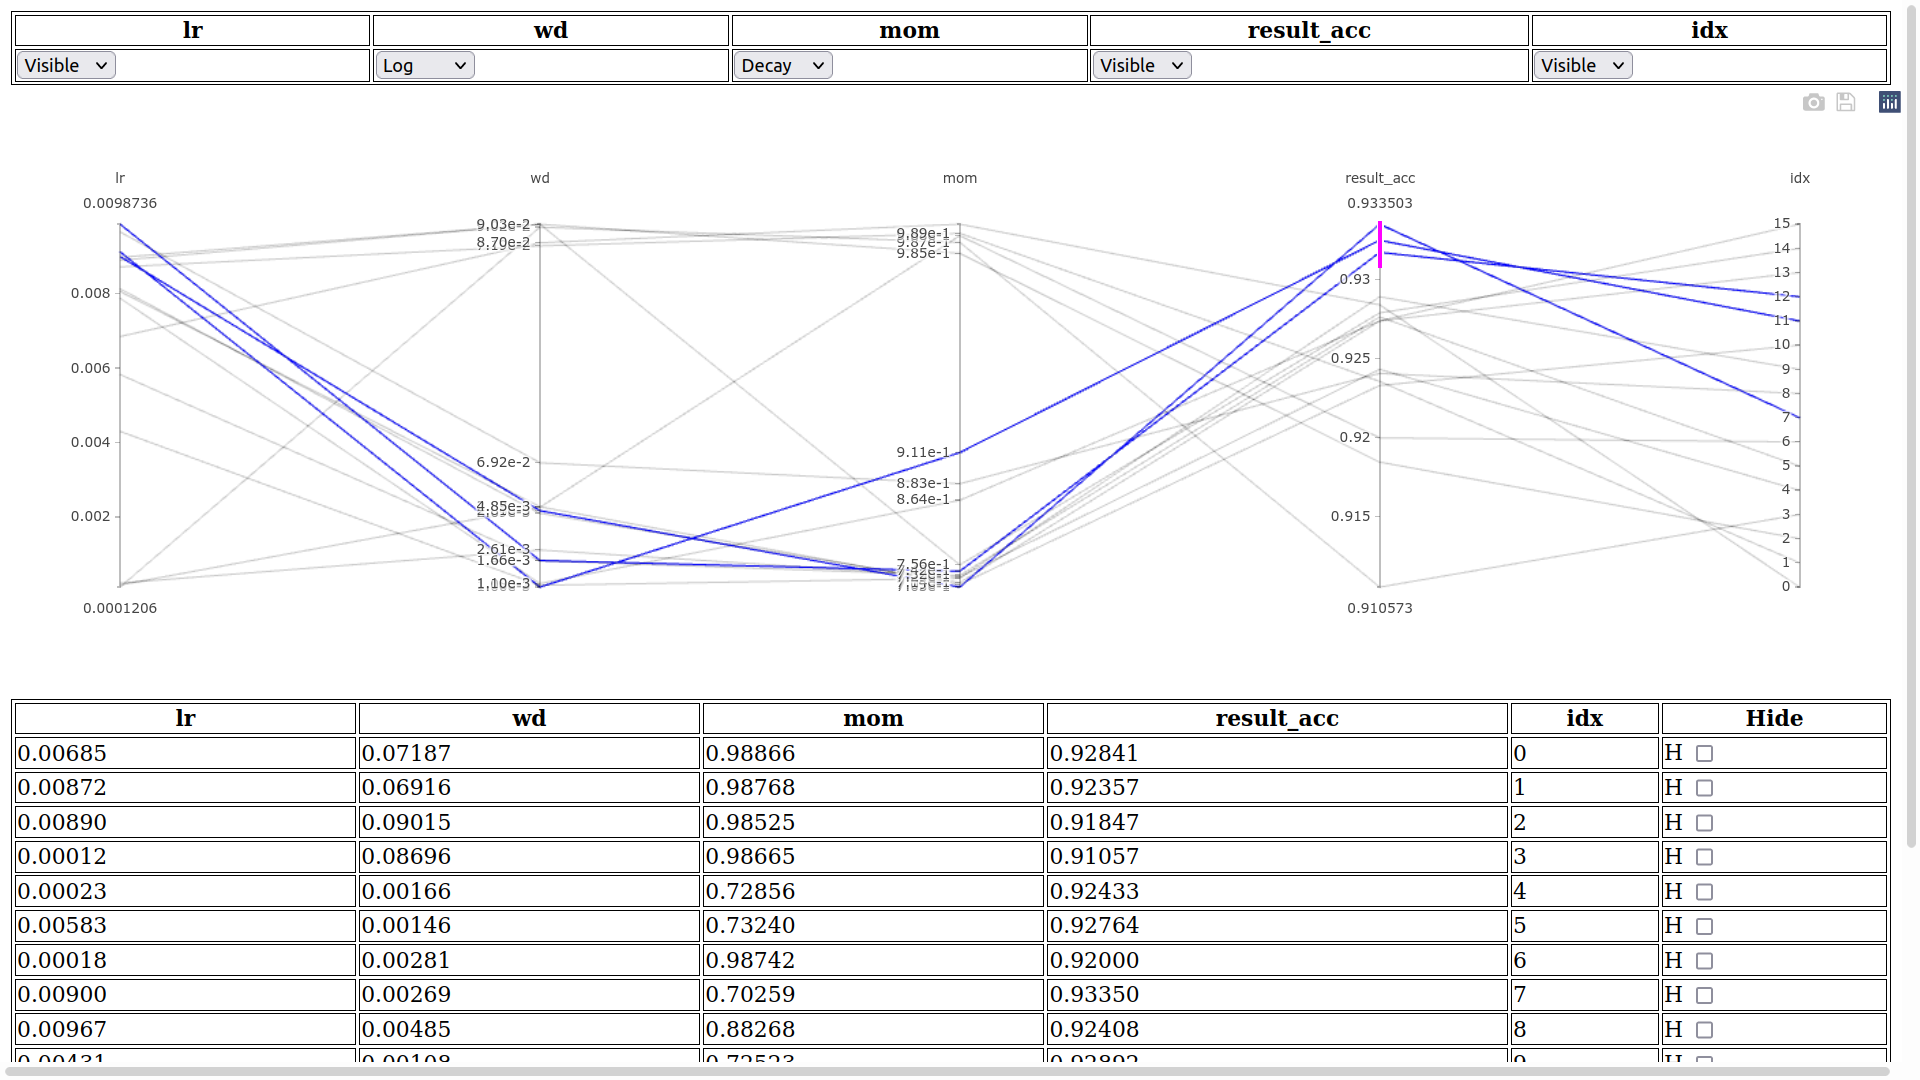
\includegraphics[width=\columnwidth]{90-files/hyper.png}
    \caption{Visualization of \texttt{torchelie.hyper} hyperparameter search. The user can select hyper parameters to sample (and how to sample them), and target metrics. Once ran, the results appear in this visualization. In this case, we highlighted via the interface the three runs with the best resulting accuracy.}
    \label{fig:tch.hyper}
\end{figure}

\paragraph{\texttt{torchelie.recipes}} a model is useless without training and inference code. Recipes are Torchélie's ways of building programs utilizing models. We provide ready to use Recipes such as CUT \cite{cut}, DeepDream \cite{deepdream}, Feature visualization for \acp{CNN} \cite{featureviz}, vanilla \ac{GAN} training \cite{gan}, image manipulations algorithms from \citet{deepimageprior}, neural style transfer \cite{styletransfer}, Pix2Pix \cite{pix2pix}, StyleGAN2 \cite{stylegan2}, and standard cross-entropy classification. Most of those recipe provide a commandline interface to complement their Python API.

\paragraph{\texttt{torchelie.callbacks}} are callbacks that can be inserted in recipes in order to instrument them with metrics, logging, additional steps, etc. They are a very powerful tool keeping the code modular and clean. We provide \texttt{Checkpoint} that saves models on disk during training, \texttt{ClassificationInspector} providing live visualization for classification models (Figure \ref{fig:classifreport}), \texttt{ConfusionMatrix} show in Figure \ref{fig:confmatrix}, various averaging strategies for logging metrics, \texttt{GANMetrics} (providing \ac{KID} \cite{kid}, \ac{FID} \cite{fid}, precision-recall \cite{precisionrecall}), \texttt{ImageGradientVis} showing the gradient magnitude of the loss wrt the input image, effectively showing the image parts that the model relied on (Figure \ref{fig:gradients}), \texttt{Polyak} (exponential) averaging of models used for instance in StyleGAN2, \texttt{Throughput} displaying the number of forward passes done per second during training in order to keep models' latency under scrutiny, \texttt{Optimizer} running an optimizer step with configurable features (such as gradient accumulation, lr logging, gradient centralization, gradient clipping), \texttt{LRSched} for lr schedulers, and some more utilities.

\begin{figure}[h]
    \centering
    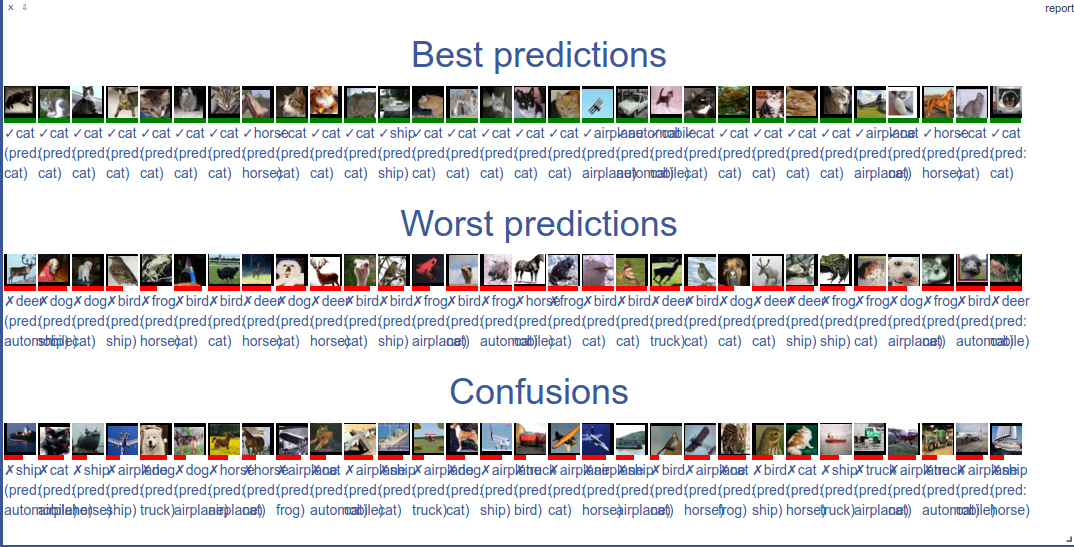
\includegraphics[width=\columnwidth]{90-files/classifreport.png}
    \caption{The \texttt{ClassificationInspector} allows to see live the performance of the classifier. It reports the samples that are provide the best, worst, and most confused answers from the classifier. The bar below the images is green when the prediction is correct, red otherwise; the width reflects the confidence score of the prediction. This allows eyeballing the datasets, strengths and weaknesses of the model, and build intuition.}
    \label{fig:classifreport}
\end{figure}

\begin{figure}[h]
    \centering
    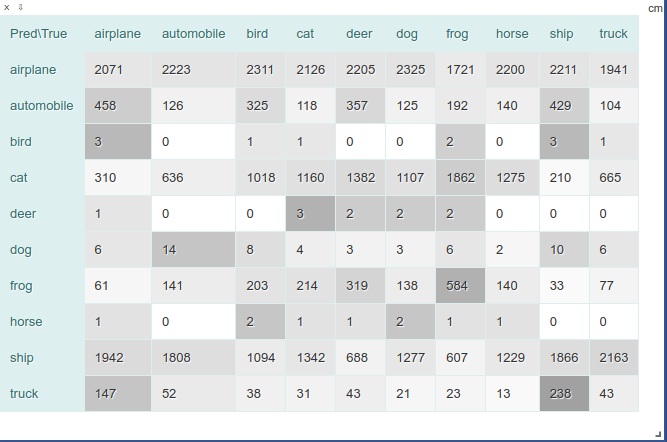
\includegraphics[width=\columnwidth]{90-files/confmatrix.png}
    \caption{Live confusion matrix provided automatically when the number of classes is not too big to make it unreadable (less than 25 classes).}
    \label{fig:confmatrix}
\end{figure}

\begin{figure}
    \centering
    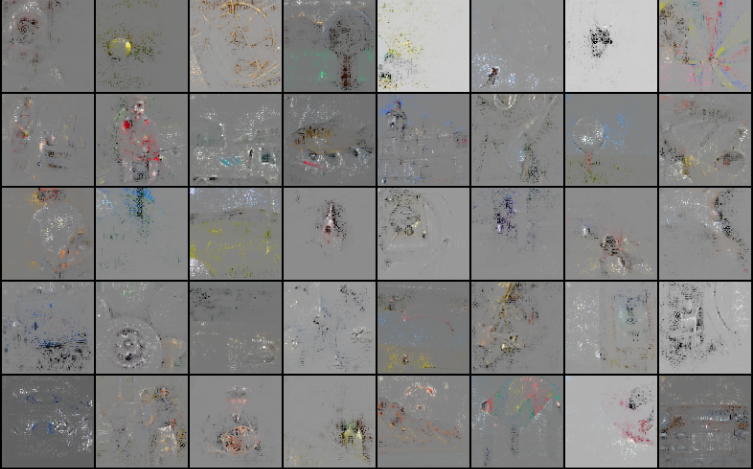
\includegraphics[width=\columnwidth]{90-files/gradients.png}
    \caption{Gradient of the loss wrt the input on the current batch. The per-pixel norm of the gradient weighs each pixel's intensity. This helps figuring out what the model looks at in the picture in order to make its predictions}
    \label{fig:gradients}
\end{figure}



\section{Design Principles}

The second contribution Torchélie proposes is a set of design patterns thought to be convenient for research and modular / incremental development and experimentation. Torchélie follows few design principles:

\begin{enumerate}
    \item \textbf{Independent} As much as possible, features must be independent and one must be able to use exactly the feature they need without difficulty. For instance, one must be able to use a layer or a model in their project and use them as much as possible as Pytorch components in their Pytorch project. One might be able to train a vanilla Pytorch model with a training loop from Torchélie without any adaptation.
    
    \item \textbf{Compositionality} Features are built by composing small and independent building blocks. All blocks must do one thing and do it well. Greater components must be designed by combining smaller components and keep the logic simple. The user should be able to easily write their own components and easily compose them to the set of feature that is looked for. For instance, it must be easy to write a new type of layer and use it in the provided models with minimal effort; to write a new metric to integrate in the training loop; to write a new training logic code; etc. This is, for instance, why our implementation of the VQVAE embodies its gradients estimator in its backward function: using this layer is now a totally local decision, there is no need to alter the code somewhere else, like in the loss function, to make it usable. 
    
    \item \textbf{Build standard and modify} This \emph{delta approach} is the new take Torchélie proposes on developping libraries. Trying to build models, training recipes, layers, with options for customization inside the object constructors leads to two kind of major issues. First, despite the best efforts, since it is very hard to know what the developer will want to control, it is unlikely that our parameters would address every implementation details. Second, the code either lacks customizability or becomes unmaintainable as one adds switches and parameters. Moreover, each layer option must be ported as well to the model's options, and the parameters and switches grow totally out of hand. In training code, this happens the same way as one might want to change a loss function, add one, etc. Instead, we should provide simple ways to build standard components, and give editing features. Instead of building customized, it is hypothesized that thinking in terms of deltas from the standard blocks scales better: the construction code remain simple and straightforward as it builds just one standard thing, and the edition functions remain external and self contained.
    
    Training code should follow the same guidelines. For instance, complex losses such as the Pix2pixHD loss should be simple but composable so that a user can easily add, remove, change or replace one term.
    
    A deep learning practitioner mainly works in incremental changes, as we evolve from a standard algorithm and evaluate their performance; let's keep these deltas expressed as deltas in the code as well.
\end{enumerate}

\subsection{Models}
\label{sec:tch.models}

Torchélie provide many architectures, that are yet to be pretrained. It provides many resnet variants and GANs architectures such as Pix2pix or StyleGAN2.

It becomes straightforward to write code in Torchelie style. The model or block is implemented in its most basic, canonical form. Derivative models are implemented in terms of transforms from those basic blocks.

Let's illustrate this first with a simple example, without using Torchélie. One wants to experiment with SE-ResNets \cite{squeezeexcitation}. In simple terms, the SE-ResNet is a ResNet which adds a Squeeze-and-Excite block in every residual layers.

A typical way to implement this, shown in Listing \ref{code:typresnet}, would be invasive changes to the ResNet definition. Implementing more and more variants would bloat the code and make it harder and harder to maintain as the code grows with switches.

\begin{figure}
\begin{lstlisting}[language=Python, label=code:typresnet, caption=Typical SE-ResNet implementation. Note how \texttt{use\_se} has to be passed down. Details are left out for clarity and brievity.]
class ResNet(nn.Module):
    def __init__(self, arch, use_se=False):
        # create input stem
        
        for n_blocks in arch:
            for i in range(n_blocks):
                self.add_module(ResBlock(..., use_se=use_se))
        # create end of trunk

class ResBlock(nn.Module):
    def __init__(self, ..., use_se=False):
        # create branch and skip convs if any
        
        if use_se:
            self.branch.add_module(SE(...))
            
se_resnet = ResNet(..., use_se=True)
\end{lstlisting}
\end{figure}

Instead, we repeat that \emph{the SE-ResNet is a ResNet which adds a Squeeze-and-Excite block in every residual layers}. This is exactly the way this should be expressed in code. The resulting code, in Listing \ref{code:deltaresnet}, is shorter, more readable, local and non invasive. There are no risks inserting bugs into vanilla resnets that were perfectly functioning before our intervention.

\begin{figure}
\begin{lstlisting}[language=Python, label=code:deltaresnet, caption=Delta implementation of SE-ResNet. There are no needs for intrusive changes.]
resnet = ResNet(...)

for m in resnet.modules():
    if isinstance(m, ResBlock):
        m.branch.append(SE(...))
\end{lstlisting}
\end{figure}


This is not cherry picking, and examples are plenty:
\begin{itemize}
    \item a Wide ResNet \cite{wrn} is "a ResNet with wider kernels". We can take a resnet, iterate on its residual blocks and replace the layers with wider ones.
    \item ResNet-v2 \cite{resnettricks} has "a ResNet with three 3x3 convs in the input stem", "a ResNet where stride 2 convolutions are the 2nd one in the branch rather than the first one", and "a ResNet that uses average pooling rather than strides in the identity path".
    \item ResNeXt \cite{resnext} uses "grouped convolutions instead of full convolutions".
    \item PoolFormer \cite{poolformer} is a Vision Transformer \cite{vit} "using average pooling instead of self attention" \cite{transformers}.
    \item ReZero \cite{rezero} "adds a learnable scalar multiplier, initialized to 0, at the end of every residual branch".
    \item etc...
\end{itemize}

Those are deltas that are easily expressed in code, and more explicitly exhibit the intent. Those deltas are fundamental for research and iterative development. Having those deltas expressed as \emph{external} transforms rather than \emph{intrusive} instrumentation is very important. To some extent, it allows modifying an architecture provided by a library without needing to alter its code. It ensures that the new delta the user is about to try does not introduce bugs into previous models and does not interfere with any other part of the code. It scales trivially as incremental changes can be layered in the exact same way, or explored in parallel, without introducing uncontrollably growing complexity with switches.

The role of \textbf{Torchélie} is to ease delta programming. This is first done by providing carefully designed interfaces:
\begin{enumerate}
    \item Models are totally described as editable computational graphs (\texttt{nn.Sequential} or \texttt{torchelie.nn.ModuleGraph}). They can be externally modified. For this, we avoid hard coded logic and hard coded design choices (there are few exceptions to this, decided with common sense). Actually, the SE-ResNet example could not have been done using \texttt{torchvision}'s definition because the contents of the residual branch is not editable in their implementation.
    \item Layers bear a semantic name, so that they can be easily and robustly indexed.
    \item  Layers that form a semantic units are grouped, so that models are not a flat sequence of fundamental operations, but a (fully editable) hierarchy exhibiting design choices; for instance, Conv-BN-ReLU are grouped together in a \texttt{torchelie.nn.ConvBlock}.
\end{enumerate}

Second, Torchélie provides utilities easing delta edition. For instance, in \texttt{torchelie.nn.utils}, we provide:

\begin{description}
    \item[\texttt{insert\_after(base, key, new, new\_name)}] that inserts \texttt{new} with name \texttt{new\_name} into model \texttt{base} after the module indexed by \texttt{key}
    \item[\texttt{insert\_before}(base, key, new, new\_name)] works similarly
    \item[\texttt{make\_leaky(m)}] that changes ReLUs in \texttt{m} into LeakyReLUs and accordingly adapts the initialization the layer before it (if applicable)
    \item[\texttt{edit\_model(model, f)}] that recursively transforms every module \texttt{m} of \texttt{model} to \texttt{f(m)}, etc.
\end{description}


\subsection{Algorithms}

Those design guidelines apply to algorithm implementation as well. This is not as straightforward as for models since we are already used to models being described as data structures. For code, we needs carefully designed code architecture.

Let's study examples of how that would work out on concrete cases.

\begin{itemize}
    \item StyleGAN2 \cite{stylegan2} (besides architectural changes) "adds a Perceptual Path Length regularizer and a R1 regularizer to a standard \ac{NSGAN}".
    \item StyleGAN2-ADA \cite{stylegan2ada} "inserts differentiable data augmentation before feeding real and fake images to the discriminator".
    \item ResNet-RS \cite{resnetrs} propose to improve resnets by "architecture improvements" (dealt with model delta programming) and "better regularization methods: adding model exponential averaging \cite{polyak} (Polyak averaging), label smoothing \cite{inceptionv2}, RandAugment \cite{randaugment} and a lower weight decay".
    \item Similarly, ResNet-SB proposes to "replace cross-entropy with \ac{BCE}, add mixup \cite{mixup} and cutmix \cite{cutmix}, use the LAMB optimizer \cite{lamb} with bigger batch size, and a few other hyper parameter differences"
    \item Pix2Pix \cite{pix2pix} "adds a L1 per pixel loss to the adversarial loss of a standard cGAN \cite{cgan}".
    \item Pix2PixHD \cite{pix2pixhd} "removes the L1 pixel loss but adds a feature matching loss and changes the \ac{NSGAN} loss to a \ac{LSGAN} loss".
    \item etc
\end{itemize}

Again, all those paper are defined in deltas from another paper or standard procedure. And even if they propose significant changes (like ResNet-SB), they came to those lists of changes by incremental trials, building deltas one on top of another, often made explicit through ablation studies. ConvNeXt \cite{convnext} is a very demonstrative example showing how research advances by stacking deltas (cf. Figure \ref{fig:convnext}).

The reasoning is the same as for handling model variants: as one adds options and wants to experiment, the code grows out of hands, and all those intrusive changes risk introducing regression bugs. Listing \ref{code:timm-params} shows how \texttt{timm} \cite{timm}, a famous library providing vision models and their training code, grew an enormous list of parameters by not following a delta approach. Developping new ideas outside of what is permitted by those is not possible without intrusive intervention inside \texttt{timm}'s code. However, humility is needed as \texttt{timm} sprung many works and supports a much much larger number of projects than Torchélie does.

\begin{figure}
\begin{lstlisting}[language=Python, label=code:timm-params, caption=Arguments to the training script of \texttt{timm}.]
(aa=None, amp=False, apex_amp=False, aug_splits=0, batch_size=32, bn_eps=None, bn_momentum=None, bn_tf=False, channels_last=False, clip_grad=None, color_jitter=0.4, cooldown_epochs=10, crop_pct=None, cutmix=0.0, cutmix_minmax=None, data_dir='../imagenette2-320', dataset='', decay_epochs=30, decay_rate=0.1, dist_bn='', drop=0.0, drop_block=None, drop_connect=None, drop_path=None, epochs=200, eval_metric='top1', gp=None, hflip=0.5, img_size=None, initial_checkpoint='', input_size=None, interpolation='', jsd=False, local_rank=0, log_interval=50, lr=0.01, lr_cycle_limit=1, lr_cycle_mul=1.0, lr_noise=None, lr_noise_pct=0.67, lr_noise_std=1.0, mean=None, min_lr=1e-05, mixup=0.0, mixup_mode='batch', mixup_off_epoch=0, mixup_prob=1.0, mixup_switch_prob=0.5, model='resnet101', model_ema=False, model_ema_decay=0.9998, model_ema_force_cpu=False, momentum=0.9, native_amp=False, no_aug=False, no_prefetcher=False, no_resume_opt=False, num_classes=None, opt='sgd', opt_betas=None, opt_eps=None, output='', patience_epochs=10, pin_mem=False, pretrained=False, ratio=[0.75, 1.3333333333333333], recount=1, recovery_interval=0, remode='const', reprob=0.0, resplit=False, resume='', save_images=False, scale=[0.08, 1.0], sched='step', seed=42, smoothing=0.1, split_bn=False, start_epoch=None, std=None, sync_bn=False, torchscript=False, train_interpolation='random', train_split='train', tta=0, use_multi_epochs_loader=False, val_split='validation', validation_batch_size_multiplier=1, vflip=0.0, warmup_epochs=3, warmup_lr=0.0001, weight_decay=0.0001, workers=4)
\end{lstlisting}
\end{figure}

Torchélie proposes tooling in order to describe code as data structures and ease delta programming of algorithms. Our currently proposed tool is the \texttt{Algorithm} class. It is an improved sequence of named functions. Those functions are called in order when executing the Algorithm. The names allow to easily manipulate the sequence in order to replace or remove existing functions, or insert new ones. That way, algorithms can be described in atomic steps that can be incrementally manipulated to grow more sophisticated or fork variants.

Let's illustrate how a standard conditional GAN algorithm can be manipulated to create new derivative algorithms, namely WGAN-GP, Pix2Pix and Pix2PixHD with small deltas.

A conditional GAN concatenates the source and target image to the discriminator. The Generator (G) pass is made in two steps: generate some fakes and compute the loss; then backpropagate to the generator. Listing \ref{code:cgang} illustrates our delta programming approach using \texttt{Algorithm} for the generator. We can see that a conditional GAN loss is defined as a pass for G and the Discriminator (D). G's include one \texttt{'fake'} step, generating fake samples, \texttt{'adversarial'} discriminating those fakes, and \texttt{'backward'} running the back propagation. Same goes for D. 

Listing  \ref{code:cgand} illustrates the steps involved in training the discriminator: \texttt{'gen\_fakes'} generates fake samples from G, \texttt{'fake\_adversarial'} computes the discriminator's output on them, \texttt{'fake\_backward'} backpropages the fake loss, \texttt{'real\_adversarial'} computes the discriminator's output on real samples and \texttt{'real\_backward'} backpropagates the loss for them. These sequences of operations are now manipulable as data from \texttt{G\_alg} and \texttt{D\_alg} members.

\begin{figure}
\begin{lstlisting}[language=Python, label=code:cgang, caption=The generator pass for a ConcatConditionalGAN. The implementation details are removed in order to focus on the design principles. The discriminator's pass is in Listing \ref{code:cgand}]
class ConcatConditionalGANLoss:
    def __init__(self, G: nn.Module, D: nn.Module) -> None:
        self.G = G
        self.D = D
        self.gan_loss = tch.loss.gan.standard

        G_alg = Algorithm()

        @G_alg.add_step('fake')
        def G_fake_pass(env, real, target):
            # Generate some fakes
            
        @G_alg.add_step('adversarial')
        def G_adv_pass(env, real, target):
            # compute the discriminator loss

        @G_alg.add_step('backward')
        def backward(env, real, target):
            # backward the discriminator loss

        self.G_alg = G_alg
        
        ...  # D's pass to be implemented here
\end{lstlisting}
\end{figure}

\begin{figure}
\begin{lstlisting}[language=Python, label=code:cgand, caption=The discriminator for a ConcatConditionalGAN. The implementation details are removed in order to focus on the design principles. The generator pass is in Listing \ref{code:cgang}]
class ConcatConditionalGANLoss:
    def __init__(self, G: nn.Module, D: nn.Module) -> None:
        ...  # G's pass to be implemented here
        
        D_alg = Algorithm()

        @D_alg.add_step('gen_fakes')
        def gen_fakes(env, real, target):
            # Generate fake images, store them in env['fake_image']

        @D_alg.add_step('fake_adversarial')
        def D_fake(env, real, target):
            # Compute the discriminator loss for fake samples.
            
        @D_alg.add_step('fake_backward')
        def D_backward(env, real, target):
            # Backpropagate the fake loss. Return some metrics

        @D_alg.add_step('real_adversarial')
        def D_real(env, real, target):
            # Compute the discriminator loss for real samples.
            
        @D_alg.add_step('real_backward')
        def D_backward(env, real, target):
            # Backpropagate the real loss. Return some metrics

        self.D_alg = D_alg

    def G_step(self, real: torch.Tensor, target: torch.Tensor) -> dict:
        return self.G_alg(real, target)

    def D_step(self, real: torch.Tensor, target: torch.Tensor) -> dict:
        return self.D_alg(real, target)
\end{lstlisting}
\end{figure}

A first variant, a conditional WGAN, could use the WGAN-GP regularizer \cite{wgangp}. This could be achieved by adding a gradient penalty computation before performing the backpropagation on D, as shown in Listing \ref{code:wgangp}. We first make sure that the GAN's \texttt{Algorithm} is using a standard \ac{BCE} loss, we define our gradient penalty, and we insert a new step in the algorithm \texttt{'D\_gp'}, right before the \texttt{'real\_adversarial'} step. The actual implementation of the gradient penalty is totally irrelevant to the point shown here: our cWGAN-GP is grown by adding a simple term, a simple delta, to our vanilla cGAN.

\begin{figure}
\begin{lstlisting}[language=Python, label=code:wgangp, caption=ConcatConditionalGAN with WGAN-GP regularizer]
def to_wgangp(cgan, gp_gamma):
    cgan.gan_loss = tch.loss.gan.standard
    gradient_penalty = GradientPenalty(gp_gamma)

    @cgan.D_alg.insert_before('real_adversarial', 'D_gp')
    def D_gp(env, real, target):
        g_norm = gradient_penalty(cgan.D, env['real_pair'], env['fake_pair'])
        return {'g_norm': g_norm}
\end{lstlisting}
\end{figure}

We can try further and implement Pix2Pix's loss instead of WGAN-GP. Pix2Pix extends the standard conditional GAN with a L1 loss between the generated picture and the actual target picture. Inheritance can achieve this and is another valid way of implementing our goal. Listing \ref{code:pix2pix} exhibits this implementation, adding the L1 term to our vanilla cGAN, the \texttt{'l1'} step, after \texttt{'real\_adversarial'}.

\begin{figure}
\begin{lstlisting}[language=Python, label=code:pix2pix, caption=Pix2Pix from ConcatConditionalGAN]
class Pix2PixLoss(ConcatConditionalGANLoss):
    def __init__(self, G: nn.Module, D: nn.Module, l1_gain: float) -> None:
        super().__init__(G, D)
        self.l1_gain = l1_gain

        @self.G_alg.insert_after('real_adversarial', 'l1')
        def G_l1_pass(env, real, target):
            loss = self.l1_gain * F.l1_loss(env['fake_image'], target)
            env['loss'] += loss
            return {'l1_loss': loss.item()}
\end{lstlisting}
\end{figure}

Pix2PixHD can be implemented as a derivative work that mostly incorporates a feature matching loss to the standard conditional GAN setting and switches to the Least-Squares GAN loss they find more stable. Listing \ref{code:pix2pixhd} implements Pix2PixHD's loss by adding \texttt{'extract\_features'} and \texttt{'feature\_matching'} before \texttt{'fake\_adversarial'}, which extract deep features from the discriminators, compute the deep feature matching loss. It finally replaces \texttt{'fake\_adversarial'} in order to compute the discriminator loss from the features instead of the default step that runs a full forward pass on D, saving compute.

\begin{figure}
\begin{lstlisting}[language=Python, label=code:pix2pixhd, caption=Pix2PixHD]
class Pix2PixHDLoss(ConcatConditionalGANLoss):

    def __init__(self, G: nn.Module, D: nn.Module, l1_gain: float):
        super().__init__(G, D)
        self.gan_loss = tch.loss.gan.ls
        self.l1_gain = l1_gain

        D_with_acts = tnn.WithSavedActivations(D.module)

        @self.G_alg.insert_before('fake_adversarial', 'extract_features')
        def G_features(env, real, target):
            # Generate fake samples, compute D's activations and its final
            # predicted probability

        @self.G_alg.insert_after('extract_features', 'feature_matching')
        def G_featmatch(env, real, target):
            # Compute the feature matching loss

        @self.G_alg.override_step('fake_adversarial')
        def G_adv(env, real, target):
            # add the actual adversarial loss
\end{lstlisting}
\end{figure}

We believe this programming paradigm highlights the incremental nature of the works, and make them easily manipulable. Easy experiments can be conducted if one wishes to remove, replace, or add elements to losses or more complex algorithms.

Torchélie's \texttt{Algorithm} class is certainly not a silver bullet, but while we believe our implementation has flaws and certainly has cases that it does not handle in a comfortable and elegant way, we are confident that this delta programming is an important paradigm for research and deep learning work in general.

\begin{figure}[h]
    \centering
    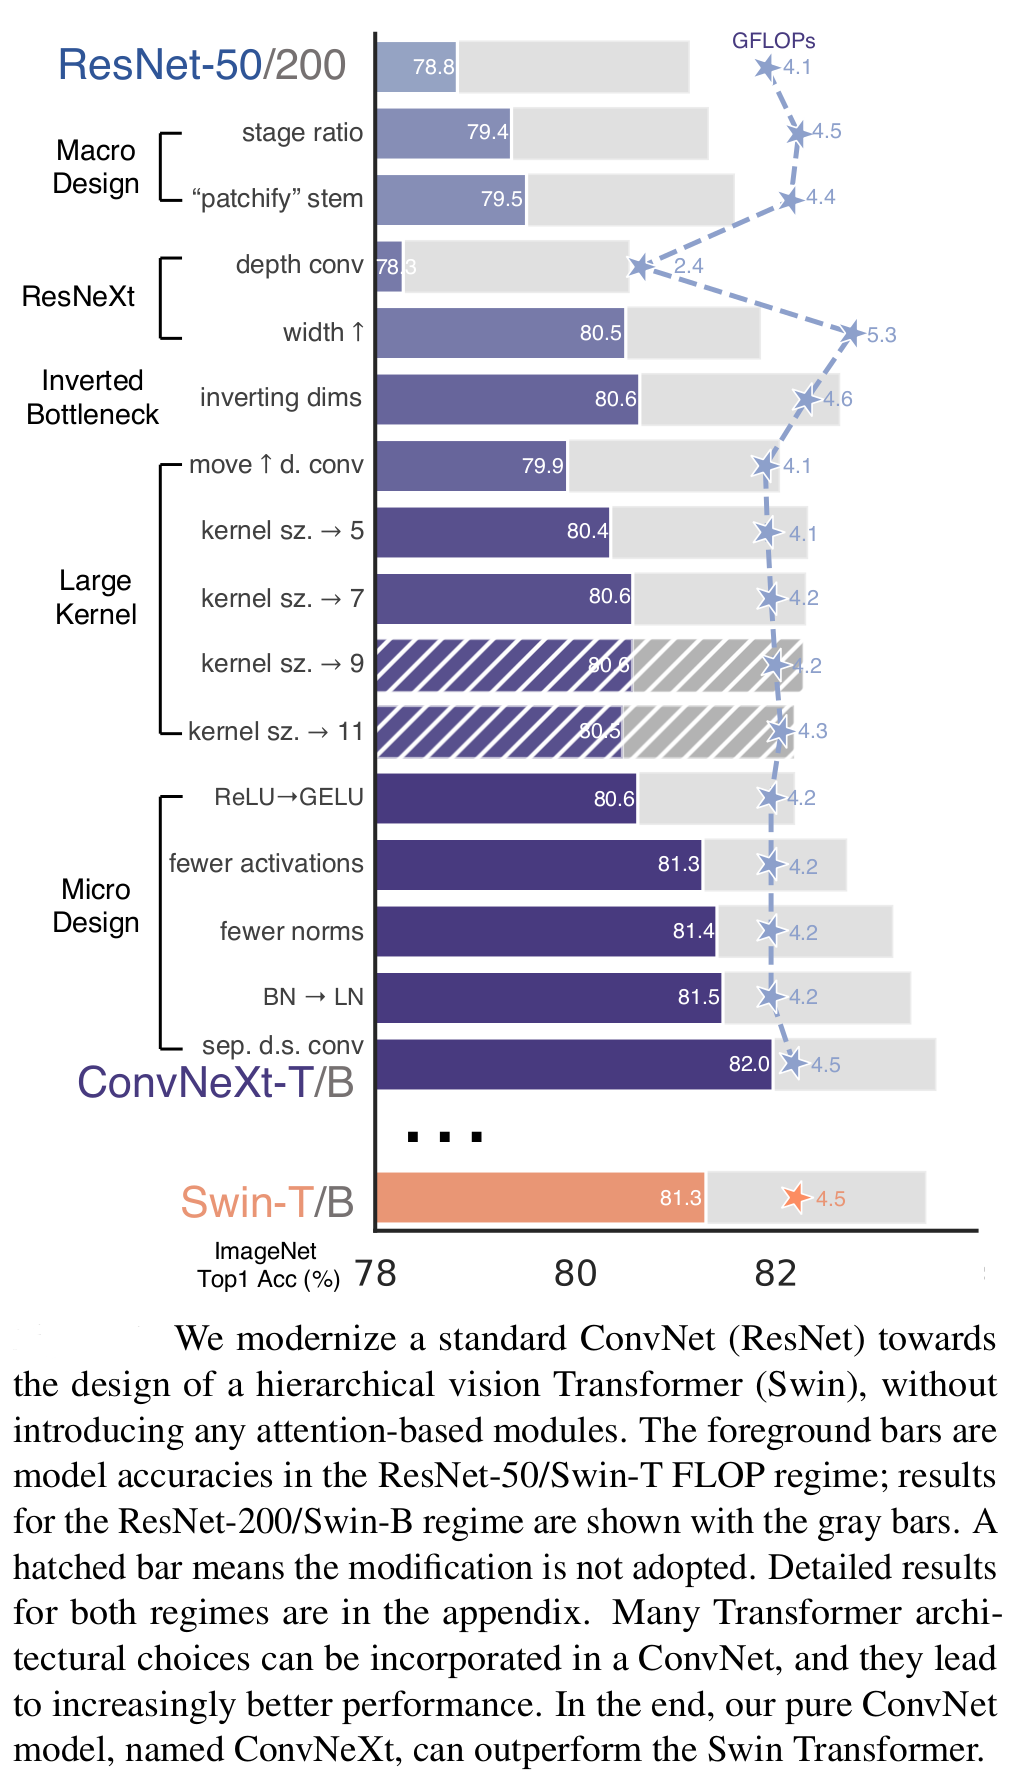
\includegraphics[width=0.7\columnwidth]{90-files/convnext.png}
    \caption{Incremental improvement process from ResNet to ConvNext. Figure extracted from \citet{convnext}.}
    \label{fig:convnext}
\end{figure}

\section{Discussion}

\subsection{The future of Torchélie}

It first important to remind that Torchélie is a tool tailored to and built from \emph{my} needs but could be useful to the community thanks to its MIT license. Having a bigger user base and more regular contributors would be very nice, but that would make modifying the library to adapt my needs harder and slower. I would now have to worry about API stability, breaking changes, etc. This \emph{is} envisioned, but for now, I consider some Torchélie parts still unstable and in alpha, often modified with design changes that would invalidate work based on it. The main cause of instability is the ongoing exploration for better tools to help delta programming for algorithms. Actually, the algorithms / recipes implemented \emph{before} the rise of the delta paradigm in Torchélie will be rewritten, and their current API will be broken. Delta programming for models is already stable and fully functional.

The library is also in need of a new scope definition. Initially, I saw Torchélie as "everything computer vision", which is now unsustainable. While it was doable at its birth to follow along the major publications in order to implement a wide range of architectures, this is not doable anymore. Torchélie needs to focus on its raison-d'être, which is research for applied industrial problems and its constraints: models trainable in a small amount of time on commodity hardware, with small or moderately sized datasets (fine tuning is another topic). This means that Torchélie only needs to implement models, tools and algorithms that passed the hard test of time, instead of the latest trend; applied to Vision Transformers \cite{vit} for instance this means implementing only the milestone models that resisted industrial testing, time, and are commonly used in benchmarks. It certainly means lagging behind, but it also means providing healthy defaults.

This project has no end, but the near future to-do list contains a lot already. First and foremost, Torchélie has focused a lot on convolutional architectures which has become less and less relevant: ResNets work well, and every other architecture I tested and implemented did not satisfy me more than ResNets. Some were just slower, and others did not deliver the expected gains. That said, another component that has been overlooked in Torchélie is in great need of implementation: the library is not up to date with modern training settings and need to implement those in convenient ways. Besides, as Python is a quite volatile language due to its dynamic typing, annotating type hints and checking them with \texttt{mypy} \cite{mypy} is an ongoing work.

\subsection{The competition}

Torchélie lives in the land of deep learning libraries, having already many competitors. The use case for Torchélie could be questioned now that other libraries such as timm \cite{timm}, Fastai \cite{fastai}, Ignite \cite{ignite}, or PyTorch-Lightning are getting traction.

\begin{enumerate}
    \item timm provides a very large quantity of models, most of which are also pretrained on ImageNet. However, its scope remains focused on training image classifiers.
    \item Fastai is closer in its scope to Torchélie. Fastai has some different design choices that makes it feel like learning an entirely novel library. Fastai mostly sits on top of Pytorch and bring its own design principles, rather than extending PyTorch horizontally.
    \item Finally, Ignite and PyTorch-Lightning are source of inspiration and close to what I envision. Torchélie tries to be more task oriented at the cost of flexibility, and fit my needs better.
\end{enumerate}

In the long run, the broad scope of Torchélie does not seem sustainable and should either narrow its scope (which has been discussed) or integrate at least parts of the aforementioned libraries in order to remain relevant with a sustainable work load. The field is advancing at an increasing pace and more means are needed today to keep up with the pace than when it started.

\section{Conclusion}

In this chapter, we presented Torchélie, a PyTorch library gathering the code (layers, losses, algorithms, training loops, etc) under a consistent and coherent Python package. We presented the double contribution that Torchélie is: 1) a toolbox for the deep learning practitioner (especially in the domain of computer vision) with a brief presentation of its content, and 2) a programming paradigm that we call \emph{Delta programming} encouraging code and models designed as data structures for extrusive and incremental modifications; illustrated with a GAN example.

We discussed the work that remained to be done on Torchélie in order to keep it relevant in the near future and more easily maintainable while maximizing its usefulness. I expressed my decision to limit the scope of new additions to models and algorithms that succeed the test of time and invest on them rather than chasing every new development in the literature. This is undoable and brings little value in the not so uncommon case where there are no influential subsequent work in my line of work. This would also help finding Torchélie's place in a rapidly growing ecosystem, maybe reusing and delegating some of its component to other packages in the PyTorch landscape like Albumentations \cite{albumentations} for image augmentation.

The main thing that could benefit Torchélie is having a community, which is at odds with its API moving fast and breaking often. This would alleviate the weight of maintaining the code.

All in all, Torchélie is an invaluable tool for both my academic and industrial work. There is a virtuous double-way feedback loop at play: Torchélie helps my works and its use allows me to figure out the tools and designs needed in the library. This symbiotic flow also allows to proof test the code and ensure its correctness and performance.


